%%%%%%%%%%%%%%%%%%%%%%%%%%%%%%%%%%%%%%%%%%%%
% Chapitre 1
%%%%%%%%%%%%%%%%%%%%%%%%%%%%%%%%%%%%%%%%%%%%

\chapter{The Hubble-Lema\^itre fragmented model} 
\label{ChapterHL}

\section{How to build a Hubble-Lema\^itre model}

\subsection{Initial state}

The first step to obtain a HL-fragmented model is to build an uniform sphere model. The N stars, depending on the required membership, have to be distributed randomly in space inside a certain radius, producing an uniform density. This can be achieved by sampling separately the distance to the center and the angular position of each star, in a method analog as used in \cite{Aarseth1974} for a Plummer model. The distance to the center should be sampled from the function:

\begin{equation}
f_R(X) = R_0 X^2
\end{equation} 

With $R_0$ the bouding radius and X a random variable following a uniform probability law between 0 and 1. A direct uniform law for the radius would overpopulate the outer regions. The angles $\phi$ and $\theta$, respectively azimuthal and polar angle in the physics convention, should be sampled from:


\begin{align}
f_\phi(X_1) & = 2\pi X_1\\
f_\theta(X_2) &= \arccos{ (X_2) }
\end{align}

With $X_1$ following a uniform probability law between 0 and 1 and $X_2$ between -1 and 1. The cartesian coordinates are then found:

\begin{align}
x &= R \sin{\theta} \cos{\phi}\\
y &= R \sin{\theta} \sin{\phi}\\
z &= R \cos{\theta} \\
\end{align}

The N particles are then homogeneously distributed in space in a sphere of radius $R_0$. The next step is to attribute velocities. Unlike other models like the Plummer model, the velocities are here straightforward. We use the well known velocity field of neighbouring galaxies: velocities are radial from the Milky Way, larger with increasing distances, taking the form:
\begin{equation}
\bold{v} =  \textrm{H}_0 \bold{r},
\end{equation}
with H$_0$ being an equivalent of the well-known Hubble parameter. For historical accuracy, I added the name of Georges Lema\^itre when I named my model. It has now been shown that the astronomical observations of redshifted galaxies and its interpretation as the consequence of an expanding universe predated Hubble's paper \citep{Hubble1929}. Georges Lema\^itre had published his conclusion on an expanding universe two years earlier \citep{Lemaitre1927}. The account of this can be found in \cite{Kragh2003,VanDenBergh2011} and \cite{Freeman2015}.

An appropriate H$_0$ to obtain a fragmented subvirial model has to be inferior to 1.4 (see next section). The model obtained from this is then evolved through a nbody integrator, which in my case is NBODY6.


\subsection{Fragmentation}

The cluster expands, driven by the initial Hubble-Lema\^itre velocity field. During this expansion, poissonian fluctuation in density from the uniform model starts to grow: the part of the cluster with more mass initially attract more stars, forming clumps, clumps merge, spontaneously building substructure. These clumps will be analyzed in another section. If H$_0$ is well chosen, the expansion stops at some point, the initial kinetic energy has been spent and converted to potential energy: the cluster is now larger, substructured and subvirial, about to collapse. The time of the end of the expansion and the critical value of H$_0$ can be derived from Newton's second law applied to an expanding spherical shell of matter.

We start from a uniform sphere of radius $R_0$, total mass $M$. We consider spherical shells as mass elements, situated at distance $r$ from the origin. As previously said, they are attributed a radial velocity following (for the shell at $r=R_0$) $\vec v_0 = \Hub_0 \vec R_0 = \Hub_0 R_0 \vec u_r$. We want to follow the radial motion of the last shell of mass m, situated at $R$ from the origin. Newton's second law gives:


%\begin{equation}
\begin{align}\label{eq:newton}
m \frac{dv}{dt} & = - \frac{G M m}{R^2}
\end{align}
%\end{equation}

By multiplying on both sides by $v$ and integrating between a given time and $t=0$, one finds:

\begin{equation}
v^2(t) - v^2_0 = 2GM \left( \inv{R} - \inv{R_0} \right)
\end{equation}

Which becomes, by taking $\nu = v/v0$,  $x= R/R0$ and $E_\ast = \frac{2GM}{R_0 v_0^2}$, which is a dimensionless measure of the total energy of the system:

\begin{equation}
\nu^2  = 1 + E_\ast \left( \inv{x} - 1 \right) .
\end{equation}

The evolution of the system has 3 outcomes, depending on the value of $E_\ast$:
\begin{itemize}
\item $E_\ast<1$ The velocity is always strictly positive as the system expands ($x->\infty$). The system is unbound.
\item $E_\ast=1$ The velocity approaches zero as the system expands. The expansion "stops at an infinite radius". The system is marginally bound.
\item $E_\ast>1$ The velocity reaches zero for a finite radius, the system is bound and will collapses back on itself once the expansion stops. 
\end{itemize}

We only consider in the following the case in which $E_\ast<1$. We have the expression

\begin{equation}
\nu = \sqrt{1+E_\ast\left(\inv{x} - 1\right)}
\end{equation}

Taking the time derivative gives:

\begin{equation}
\frac{d \nu}{dt} = - \frac{E_\ast}{2 x^2} \left[ 1 + E_\ast\left(\inv{x} -1\right)\right]^{-\frac{1}{2}} \frac{dx}{dt}
\end{equation}

Combining this with (\ref{eq:newton}), one obtains:

\begin{equation}
\frac{dx}{dt} = \Hub_0 \sqrt{1+ E_\ast\left( \inv{x} -1\right)}
\end{equation}

which can be rewritten, using $\tilde{\Hub_0} = \Hub_0 \sqrt{E_\ast-1}$ and $x_t=\frac{E_\ast}{E_\ast-1}$

\begin{equation}
\frac{dx}{dt} = \tilde{\Hub_0} \sqrt{\frac{x_t}{x}-1}
\end{equation}

$x_t$ being the extent of the maximum expansion as we assumed a bound system. The subscript t is for "turn-around". If we choose the notation $u = \frac{x}{x_t}$:

\begin{equation}
\sqrt{\frac{u}{u-1}} \frac{du}{dt} = \frac{\tilde{\Hub_0}}{x_t}
\end{equation}

We know that $x$ varies from 1 to $x_t$, thus $u$ varies from $1/x_t$ to 1. We can then make the change of variable $u = \sin^2\theta$ and separate the variables:

\begin{equation}
\sqrt{\frac{\sin^2\theta}{1-\sin^2\theta}} 2 \sin\theta \cos\theta d \theta = \frac{\tilde{\Hub_0}}{x_t} dt
\end{equation}

which becomes after simplifications:

\begin{equation}
[ 1 - \cos(2\theta)]d\theta = \frac{\tilde{\Hub_0}}{x_t} dt .
\end{equation}


We now integrate the expression from $t=0$ to $t$, the time at which the expansions stops and $x$ reaches $x_t$ (wich implies $u_t = 1$ and $\theta_t = \pi /2)$:

\begin{align}
\int^{\pi/2}_{\theta_0} [ 1 - \cos(2\theta)]d\theta  & = \int^t_0 \frac{\tilde{\Hub_0}}{x_t} dt\\
\frac{\pi}{2} - \theta_0 + \frac{\sin(2\theta_0)}{2} & =  \frac{\tilde{\Hub_0}}{x_t} t\\
\pi - 2 \theta_0 + \frac{2}{\sqrt{x_t}}\sqrt{1-\inv{x_t}} & = 2 \frac{\tilde{\Hub_0}}{x_t} t 
\end{align}

which boils down to the expression of the time at which the expansion stops:

\begin{equation}
t = \frac{E_\ast \left(\frac{\pi}{2} - \theta_0\right) + \sqrt{E_\ast-1}}{\Hub_0 (E_\ast-1)^{-\frac{3}{2}}}.
\end{equation}

Recalling the quantities:
\begin{align}
E_\ast = \frac{2GM}{R_0 v_0^2}        &;  & x_t=\frac{E_\ast}{E_\ast-1}  &;  &\theta_0 = \sin^{-1}\left(\inv{\sqrt{x_t}}\right)  
\end{align}



\begin{figure}
\label{Fig:apextime}
\center
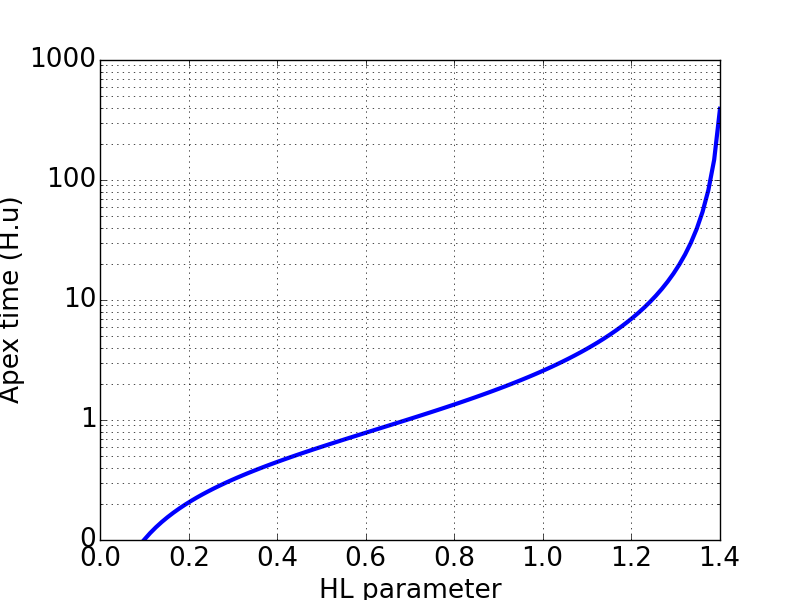
\includegraphics[width=0.7\linewidth]{Figures/1_apextime.png}
\caption{}
\end{figure} 











